\documentclass[11pt, letterpaper]{article}
\usepackage[utf8]{inputenc}
\usepackage[letterpaper, margin=0.5in]{geometry}
\usepackage{amsmath}
\usepackage{amssymb}
\usepackage{amsthm}
\usepackage{graphicx}
\usepackage[font=scriptsize]{caption}
\usepackage{subcaption}
\graphicspath{ {.} }
\captionsetup{justification=raggedright, singlelinecheck=false}


\title{STA 602 HW3}
\author{Ryan Tang}
\date{September 17th 2022}

\begin{document}
\maketitle

\section{Excerise PH 3.3}
\paragraph{(a)}
Here, we first define the prior, the generative distribution, and the general posterior for Poisson-Gamma pair.

\begin{align*}
  p(Y|\theta) &= \prod_{i=1}^{n} \frac{1}{y_i!} \theta^{y_i} e^{-\theta} && Y_{i \in n} \overset{iid}{\thicksim} Poisson(\theta) \\
    &= c(Y) \theta^{\sum y_i} e^{-n\theta}
\end{align*}
\begin{align*}
  p(\theta) &\thicksim Gamma(a, b) \\
    &= \frac{b^a}{\Gamma(a)} \theta^{a-1} e^{-b\theta}
\end{align*}
\begin{align*}
  \therefore p(\theta|Y) &\propto p(Y|\theta) p(\theta) \\
    &= \theta^{\sum y_i} e^{-n\theta} \theta^{a-1} e^{-b\theta} \\
    &= \theta^{a - 1 + \sum y_i} e^{-\theta(b+n)} \\
    &\thicksim Gamma(a + \sum_{i=1}^{n} y_i, b + n)
\end{align*}

Therefore, given $Y_A = (12, 9, 12, 14, 13, 13, 15, 8, 15, 6)$, $p(\theta_A|Y_A) \thicksim Gamma(237, 20)$.
And similiarly, given $Y_B = (11, 11, 10, 9, 9, 8, 7, 10, 6, 8, 8, 9, 7)$, $p(\theta_B|Y_B) \thicksim Gamma(125, 14)$.
The $\theta_A$ posterior has a mean of 11.85, variances of 0.593, and 95\% confidence interval of $[10.39, 13.41]$.
The $\theta_B$ posterior has a mean of 8.93, variances of 0.638, and 95\% confidence interval of $[7.43, 10.56]$.

\newpage
\paragraph{(b)}
It is hard to get the expectation of $\theta_B$ close to the $\theta_A$ posterior expectation. It only happens
after $n0$ goes over 275+, the prior sample size. Or we can also use a prior that is similar to
$Gamma(14 \times n0, n0)$ to make it easier with smaller prior sample size.

\begin{figure*}[!h]
  \centering
  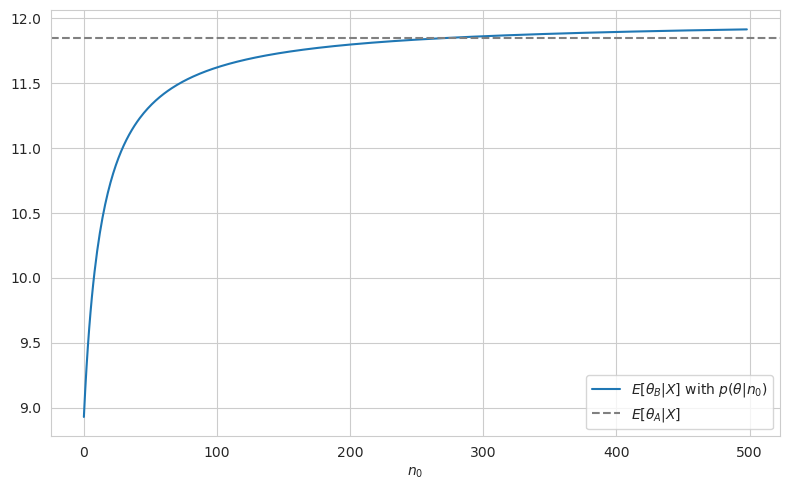
\includegraphics[width=0.8\textwidth]{3.3.b.png}
  \captionsetup{justification=centering}
  \caption{$\theta_B$ sensitivity to $n_0$}
\end{figure*}

\paragraph{(c)}
I do not think it is a good idea to transfer the knowledge from $\theta_A$ to use it in inferening $\theta_B$
based on the given information. They behave differently based on the data given. In other words,
we can assume they are conditionally independent given the data $\mathbf{X}$.
\newpage


\section{Excerise PH 3.5}
\paragraph{(a)}
As long as we model both the sampling distribution and the prior all within the exponential family, the resulting
posterior is also an exponential family distribution. The derivation also generalizes to priors that are
a mixture of exponential family distributions. The resulting posterior is a weighted average
of each prior $p(\phi)$ that is updated by the data $X$ separately with a minor tweak on the scaling constants.

\begin{proof}
Let the sampling distributions under the exponential family form be,
\begin{align*}
  p(x|\eta) &= h(x)\exp[\eta t(x) - A(\eta)] \\
  p(X|\eta)
    &= \prod_{i=1}^{n} h(x_i)\exp[\eta t(x_i) - A(\eta)]
      && X_{i \in n} \overset{iid}{\thicksim} p(x|\eta) \\
    &= (\prod_{i=1}^{n} h(x_i)) \exp[\eta \sum_{i=1}^{n} t(x_i) - n A(\eta)] \\
    &= (\prod_{i=1}^{n} h(x_i)) \exp[\eta \, n \bar{t}(X) - n A(\eta)]
      && \bar{t}(X) = \frac{1}{n} \sum_{i=1}^{n} t(x_i) \\
\end{align*}
where $h(x)$ is the scaling constant, $\eta$ is the natural parameter, $t(x)$ is the sufficient statistics,
and $A(\eta)$ is the log partition function. Then, the mixture proof be the form of
\begin{align*}
  \tilde{p}(\eta) &= \sum_{k=1}^{K} w_k p_k(\eta)
    && p_k(\eta) = \kappa(n_0^{(k)}, t_0^{(k)}) \exp[\eta \, n_0^{(k)} t_0^{(k)} - n_0^{(k)} A(\eta)]
\end{align*}
where $w_k > 0, \forall k \in K$, and $\kappa$ is the scaling constant for the prior. Hence we can write
the posterior as follow.

\begin{align*}
  p(\eta|X) &\propto p(X|\eta)\tilde{p}(\eta) \\
    &= \prod_{i=1}^n p(x_i|\eta) \cdot \sum_{k=1}^{K} w_k p_k(\eta|n_0^{(k)}, t_0^{(k)}) \\
    &= (\prod_{i=1}^{n} h(x_i)) \exp[\eta \, n \bar{t}(X) - n A(\eta)]
       \sum_{k=1}^{K} w_k \kappa(n_0^{(k)}, t_0^{(k)}) \exp[\eta \, n_0^{(k)} t_0^{(k)} - n_0^{(k)} A(\eta)] \\
    &= \sum_{k=1}^{K} w_k^{\prime} \exp[\eta(n_0^{(k)} t_0^{(k)} + n\bar{t}(X)) - (n_0^{(k)} + n) A(\eta)] \\
  w_k^{\prime} &= w_k \, \kappa(n_0^{(k)}, t_0^{(k)}) \prod_{i=1}^{n} h(x_i)
\end{align*}

Lastly, the original $p(\theta|X)$ posterior can be obtained through a change of variable.
\begin{align*}
  p_{\theta}(\theta|X) = p_{\eta}(g^{-1}(\theta)|X) \,\, |\frac{d}{d\theta}g^{-1}(\theta)| && \eta = g^{-1}(\theta)
\end{align*}
\end{proof}
\newpage

\paragraph{(b)}
\begin{proof}
First, we write the Poisson distribution in its exponential family form.
\begin{align*}
  p(x|\theta) &= \frac{1}{x!} \theta^x e^{-\theta} \thicksim Poisson(\theta) \\
    &= \frac{1}{x!} \theta^x e^{-\theta} \\
  p(x|\eta) &= \frac{1}{x!} \exp[x\eta - e^{\eta}] \\ \\
  \therefore \quad 
    & \eta = \log\theta, \quad A(\eta) = e^{\eta} \\
    & t(x) = x, \quad h(x) = \frac{1}{x!} \\
  p(X|\eta) &= (\prod_{i=1}^n \frac{1}{x_i !}) \exp[\eta \, n \bar{X} - n e^\eta]
\end{align*}
Hence, its conjugate Gamma prior has to hold the form of
$p(\eta) = \kappa(n_0, t_0)\exp[n_0 t_0 \eta - n_0 e^{\eta}]$.
With a change of variable from $\theta$ to $\eta$, we can recover the scaling constant $\kappa$ and write both $a$
and $b$ in terms of $n_0$ and $t_0$.
\begin{align*}
  p(\theta|a, b) &= \frac{b^a}{\Gamma(a)} \theta^{a-1} e^{-b\theta}
      && \theta = g^{-1}(\eta) = e^{\eta} \\
  p(\eta|a, b) &= \frac{b^a}{\Gamma(a)} e^{\eta(a-1)} e^{-b e^\eta} e^\eta \\
    &= \frac{b^a}{\Gamma(a)} \exp[\eta a - b e^\eta] \\
  p(\eta | a = n_0 t_0, b = n_0) &= \frac{n_0^{n_0 t_0}}{\Gamma(n_0 t_0)} \exp[\eta \, n_0 t_0 - n_0 e^\eta]
\end{align*}
Therefore, the gamma mixture has the following form.
\begin{align*}
  \tilde{p}(\eta) &= \sum_{k=1}^K w_k 
    \frac{{n_0^{(k)}}^{n_0^{(k)} t_0^{(k)}}}{\Gamma(n_0^{(k)} t_0^{(k)})}
    \exp[n_0^{(k)} t_0^{(k)} \eta - n_0^{(k)} e^{\eta}]
\end{align*}
Now, we can write the $\theta$ posterior through a change of variable.
\begin{align*}
  \tilde{p}(\eta|X) &\propto p(X|\eta)\tilde{p}(\eta) \\
    &= (\prod_{i=1}^n \frac{1}{x_i !}) \exp[\eta \, n \bar{X} - n e^\eta]
    \sum_{k=1}^K w_k
      \frac{{n_0^{(k)}}^{n_0^{(k)} t_0^{(k)}}}{\Gamma(n_0^{(k)} t_0^{(k)})}
      \exp[n_0^{(k)} t_0^{(k)} \eta - n_0^{(k)} e^{\eta}] \\
    &= \sum_{k=1}^K w_k^{\prime} \exp[(n_0^{(k)} t_0^{(k)} + n\bar{X}) \eta - (n_0^{(k)} + n) e^{\eta}]
      && w_k^{\prime} = w_k \frac{{n_0^{(k)}}^{n_0^{(k)} t_0^{(k)}}}{\Gamma(n_0^{(k)} t_0^{(k)})}
        (\prod_{i=1}^n \frac{1}{x_i !}) \\
  \tilde{p}_\theta(\theta|X)
    &= \sum_{k=1}^K w_k^{\prime}
      \exp[(n_0^{(k)} t_0^{(k)} + n\bar{X}) \log\theta - (n_0^{(k)} + n) e^{\log\theta}] \frac{1}{\theta} \\
    &= \sum_{k=1}^K w_k^{\prime} \theta^{n_0^{(k)} t_0^{(k)} + n\bar{X} - 1} e^{-(n_0^{(k)}+n)\theta}
\end{align*}
\end{proof}
\newpage


\section{Excerise PH 3.8}
\paragraph{(a)}
To encode the belief that 20\% of coins are symmetric and the remainings have a bias towards either head or tail, I
will arbitrarily choose a total sample size of 36 for the bias beta and 10 sample size for the symmetry beta
in the mixture assuming Diaconis and Ylvisaker should have at least examed these amounts of coin for their
statement. To be precise, the resulting prior looks like below.

\begin{align*}
  p(\theta) &\propto 0.4 Beta(12, 24) + 0.4 Beta(24, 12) + 0.2 Beta(5, 5)
\end{align*}
\begin{figure*}[!h]
  \centering
  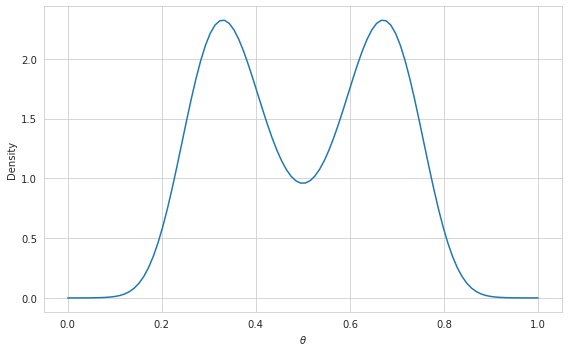
\includegraphics[width=0.6\textwidth]{3.8.a.png}
  \captionsetup{justification=centering}
  \caption{Coin Prior of $\theta$}
\end{figure*}

\paragraph{(b)}
I had a year-1999 penny tossed 50 times and obtained 29 heads, surprisingly.

\paragraph{(c)}
After incorporating the experiment data with a binomial likelihood, the resulting $\theta$ posterior for the year-1999
penny looks like the following.

\begin{figure*}[!h]
  \centering
  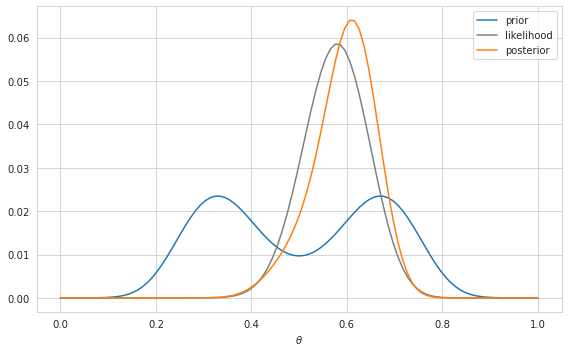
\includegraphics[width=0.6\textwidth]{3.8.c.png}
  \captionsetup{justification=centering}
  \caption{Coin Posterior of $\theta$ --- 1999 penny}
\end{figure*}

\paragraph{(d)}
After seeing the experiment result, I started to believe in Diaconis and Ylvisaker's statement more strongly.
Nevertheless, with only one sample, I do not think it is appropriate to believe that the coin denomination or the
year has anything to do with the bias. Although, the biasness indeed exists; hence, I only 1.5x times
the prior sample sizes.

\vspace{0.15in}

This time with nickel from 2013, I obtained 21 heads instead out of 50 tosses. Therefore, here is the
$\theta$ posterior for this nickel.

\begin{figure*}[!h]
  \centering
  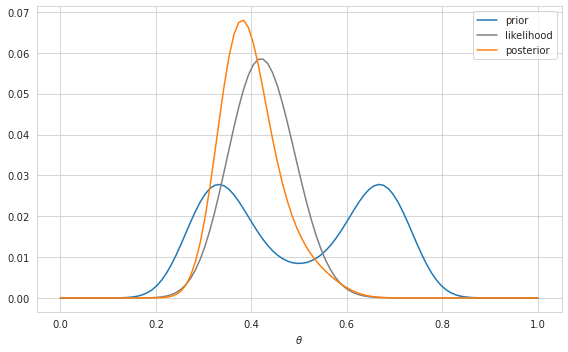
\includegraphics[width=0.6\textwidth]{3.8.d.png}
  \captionsetup{justification=centering}
  \caption{Coin Posterior of $\theta$ --- 2013 nickel}
\end{figure*}

\newpage


\section{Excerise PH 4.3}
\paragraph{(a)}
Overall the Poisson generative model matches quite well with the data, $Y_A$. 

\begin{figure*}[!h]
  \centering
  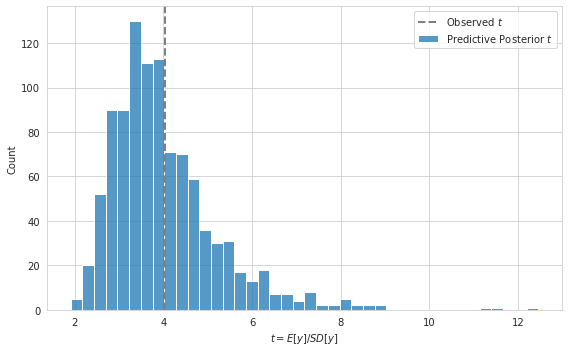
\includegraphics[width=0.8\textwidth]{4.3.a.png}
  \captionsetup{justification=centering}
  \caption{Posterior Predictive Model Check for Group A}
\end{figure*}

\paragraph{(b)}
However, the model does not work well with the group B data, $Y_B$. It could be that we have a terrible prior,
not enough data size, or perhaps Poisson is just not a good model for the data.

\begin{figure*}[!h]
  \centering
  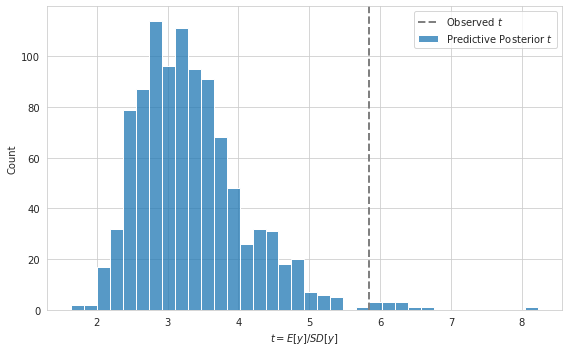
\includegraphics[width=0.8\textwidth]{4.3.b.png}
  \captionsetup{justification=centering}
  \caption{Posterior Predictive Model Check for Group B}
\end{figure*}
\newpage


\section{Excerise 5}
\paragraph{(a)}
Given the prior $\theta \thicksim Gamma(a=10, b=1)$ and the sampling model
$X_{i \in n} \overset{iid}{\thicksim} Poisson(\theta)$, the posterior is also a gamma distribution.
Now we know we received a total of 200 call from 10 different days, the posterior
\[ \theta|\mathbf{X} \thicksim Gamma(a=210, b=11) \]
The $\theta$ estimate that minimizes the L2 loss is the mean, 19.09. And the $\theta$ estimate
that minimizes the L1 loss is the median, 19.06.

\paragraph{(b)}
The model is reasonable because observing 20 calls on average is a typical belief shown in the posterior.
However, given only one data point, it is hard to tell the truth. The underlying data points might well be
$\{0, 0, \dots, 0, 200\}$. In such a case, our model performs poorly instead. In other words, if all we
care about is the average, the model is fine.

\begin{figure*}[!h]
  \centering
  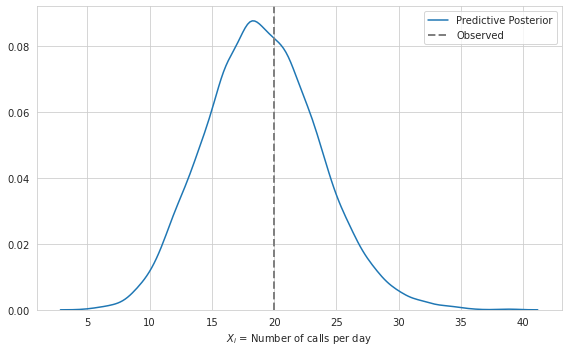
\includegraphics[width=0.8\textwidth]{5.b.png}
  \captionsetup{justification=centering}
  \caption{Posterior Predictive Model Check}
\end{figure*}
\newpage

\end{document}